% !TEX encoding = UTF-8
% !TEX TS-program = pdflatex
% !TEX root = ../tesi.tex

%**************************************************************
\chapter{Analisi dei dati}
\label{cap:Analisi}
%**************************************************************
\intro{Nel seguente capitolo verrà illustrata la fase di preprocessing e le analisi grafiche dei dati. Le analisi verranno svolte usando il linguaggio di programmazione di \autocite{R-language}. }\\

%*************************************************************

\section{Preprocessing dei dati}
Dopo aver importato il \emph{dataset}, il primo step da effettuare durante il \emph{prepocessing} è individuare e risolvere possibili anomalie nei dati.\\
Il dataset non ha valori mancanti. Questo è stato possibile grazie a \texttt{\cite{fbref}} che ha messo a disposizione dati quasi sempre completi; in quei rari casi di mancanza di dati sono stati reperiti manualmente da altre fonti altrettanto attendibili.\\ 
Sono state inoltre tolte le variabili \texttt{Date} e \texttt{Round}.\\
Il passo successivo è stato controllare che le variabili fossero interpretate correttamente. Infatti, \texttt{Team} e \texttt{Vs} vengono interpretate erroneamente come tipo \texttt{character}. Perciò, \texttt{Team} e \texttt{Vs} devono essere interpretate come un fattore cioè come un valore non numerico espresso in termini verbali, ad esempio una categoria. Quindi, nel nostro contesto ogni squadra sarà un livello del fattore. Analogamente, \texttt{AtHome} è stata trasformata in un fattore a due livelli. Invece, \texttt{Res} è stato trasformato in un fattore ordinato con i seguenti livelli.

\begin{equation}
	Res =
	\begin{cases}
		1 & \text{se la squadra in casa batte la squadra ospite,}\\
		2 & \text{se la partita termina con un pareggio,}\\
		3 & \text{se la squadra ospite batte la squadra in casa. }
	\end{cases}       
\end{equation}



\section{Analisi grafica dei dati}
In questa sezione attraverso il supporto di grafici, si analizzerà graficamente i dati disponibili e le loro relazione per avere una prima visione dei dati raccolti. Si valuteranno le relazioni tra covariate e la variabile di risposta, le relazioni tra due covariate. Tutto ciò per individuare quali covariate possano essere significative per la variabile risposta e quali interazioni emergono dall'analisi grafica.\\

Come primo passo, è stata valutata la distribuzione della variabile risposta \texttt{Res}, come è mostrato in Figura \ref{fig:res}.
\begin{figure}[htbp]
	\begin{center}
		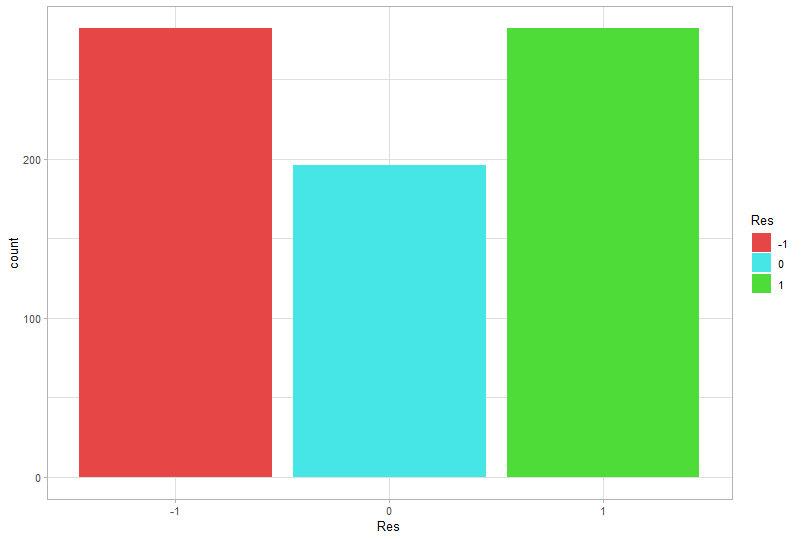
\includegraphics[scale=0.40]{barRes.png}
		\caption{Barplot della distribuzione della variabile di risposta \texttt{Res}} \label{fig:res}
	\end{center}
\end{figure}
Si può notare come le classi sembrino ben distribuite, dato che abbiamo 196 pareggi e 282 vittorie e altrettante sconfitte. Si ha quindi un campione abbastanza ampio, distribuito e privo di classi povere.\\
La Figura \ref{fig:team} mostra la distribuzione delle vittorie, dei pareggi e delle sconfitte per ogni squadra. 

\begin{sidewaysfigure} 
	\centering
	\begin{center}
		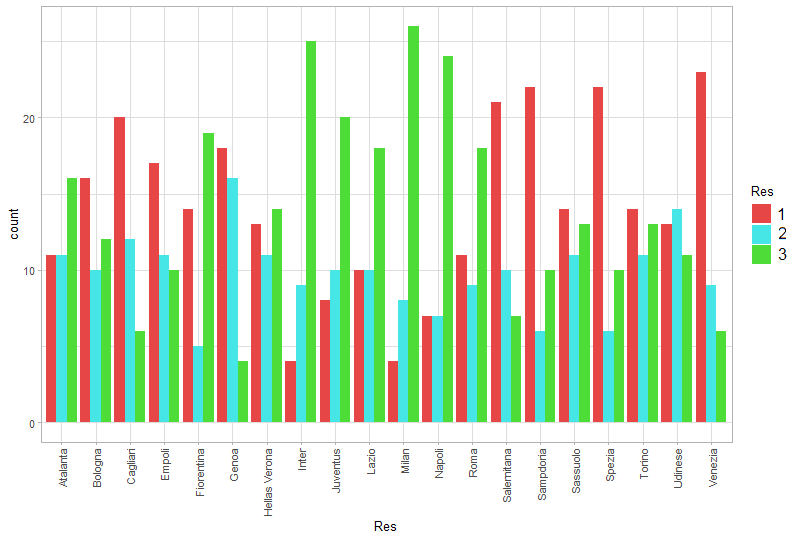
\includegraphics[height = 15cm, width = 25cm]{ResTeam.png}
		\caption{Barplot della distribuzione della variabile di risposta per squadra\texttt{Res}} \label{fig:team}
	\end{center}
\end{sidewaysfigure} 

Successivamente si è valutata la distribuzione dei gol ovvero, la frequenza del numero di gol a partita distinguendo i gol per la squadra in casa e per quella ospite. La Figura \ref{fig:goal} mostra la distribuzione del numero di gol.
\begin{figure}[htbp]
	\begin{center}
		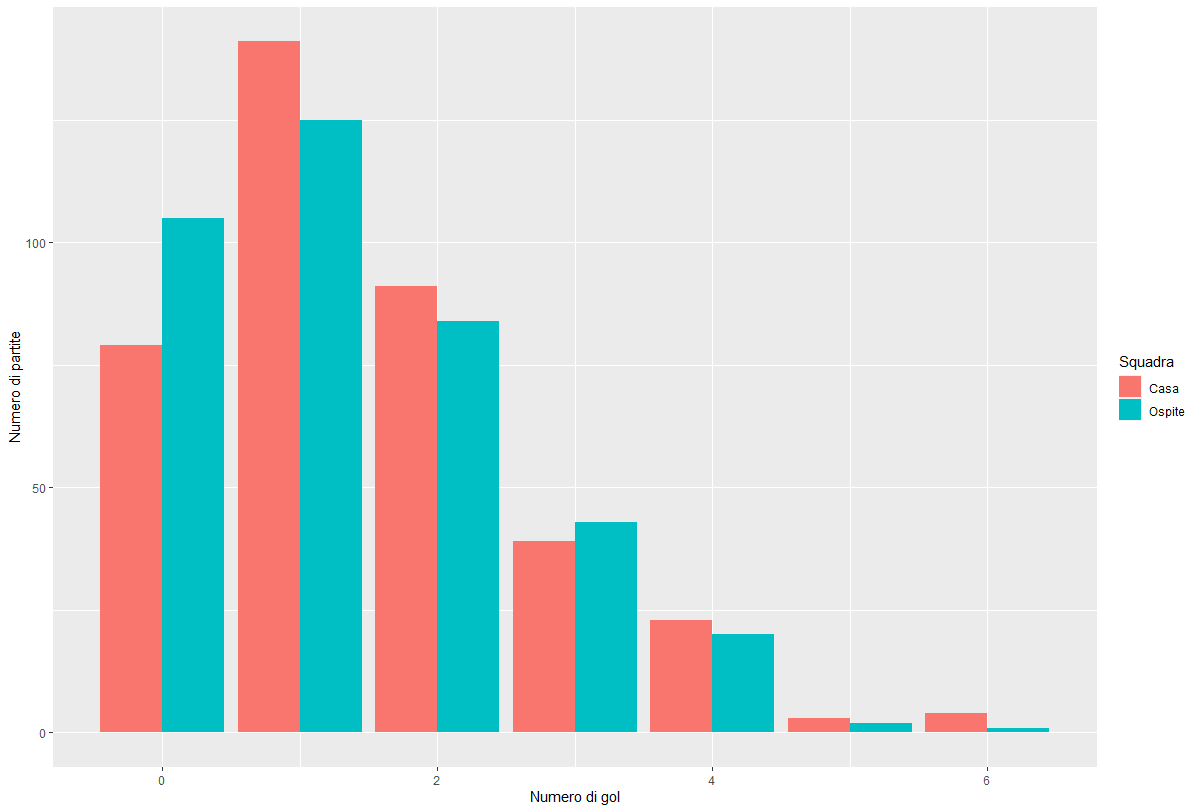
\includegraphics[scale=0.40]{goal.png}
		\caption{Barplot della distribuzione del numero di gol a partita. In azzurro vengono indicati i gol per la squadra in casa mentre in rosa i gol per la squadra ospite} \label{fig:goal}
	\end{center}
\end{figure}
Il grafico \ref{fig:goal} riporta che la squadra in casa ha segnato in più partite un gol e due gol rispetto alla squadra ospite. Inoltre, l'evento in cui la squadra in casa non segna nessun gol ha una frequenza nettamente inferiore a quella della squadra ospite. Tuttavia, si nota una certa tendenza delle partite a finire con pochi gol, al massimo due gol per squadra.
\subsection{Relazione tra la variabile risposta e le covariate}

La prima relazione che si analizza riguarda la variabile categorica \texttt{AtHome}. Nella Figura \ref{fig:AtHome} viene riportato il mosaicplot tra la variabile risposta \texttt{Res} e \texttt{AtHome}. Tale grafico è un particolare tipo di diagramma a barre impilate che mostra la relazione che c'è tra due fattori. Il numero di colonne è uguale al numero livelli della variabile inserita sull'asse orizzontale. L'altezza delle barre in verticale, invece, è proporzionale al numero di osservazioni della variabile inserita sull'asse verticale per ciascun livello della variabile nell'asse orizzontale.
In sostanza, il mosaicplot è una rappresentazione grafica di una tabella di contingenza che permette un confronto visivo tra gruppi. Nella Figura \ref{fig:AtHome} c'è una leggera variazione dei risultati tra la squadra che gioca in casa e l'avversaria, infatti per le squadre che giocano in casa, c'è una maggior presenza di vittorie e di minor sconfitte. Naturalmente non c'è alcuna variazione per il pareggio dato che entrambe le squadre lo ottengono.

\begin{figure}[htbp]
	\begin{center}
		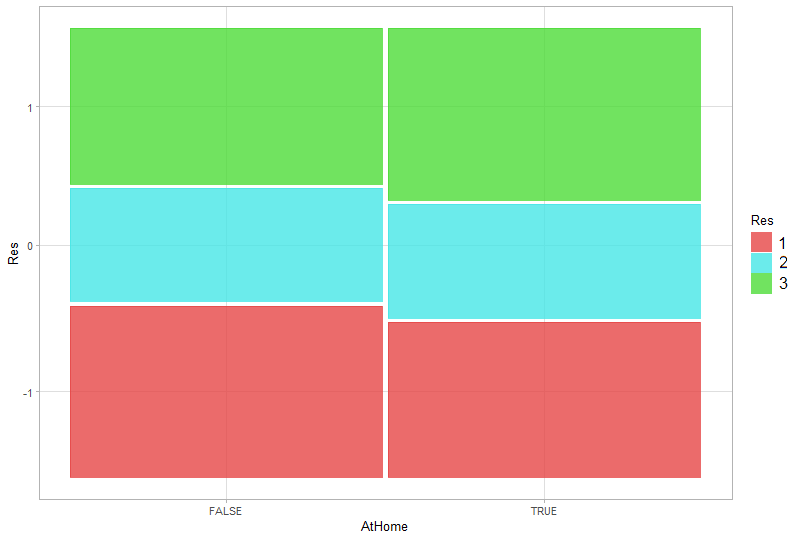
\includegraphics[scale=0.45]{AtHomeRes.png}
		\caption{Mosaicplot che mostra la distribuzione degli esiti rispetto alle partite giocate in casa e fuori casa} \label{fig:AtHome}
	\end{center}
\end{figure}

Nella Figura \ref{fig:Poss} viene riportato il boxplot della distribuzione della variabile \texttt{Poss} rispetto ai valori della variabile risposta \texttt{Res}. Il boxplot è un grafico che consente di visualizzare il centro e la distribuzione dei dati. Inoltre, può essere uno strumento visivo per la verifica della normalità o per l'identificazione di possibili outlier. Dal grafico si nota che \texttt{Poss} sembra essere significativa per l'esito. Infatti, i valori crescono dal boxplot della sconfitta al boxplot della vittoria. C'è una buona distribuzione dei dati perché la lunghezza dei baffi per ogni boxplot è simmetrica. Si segnala che la mediana della sconfitta è più vicina al 3$^{\circ}$ quantile mentre la mediana della vittoria è più vicina al 1$^{\circ}$ quantile. Non sono presenti outliers.\\
\begin{figure}[htbp]
	\begin{center}
		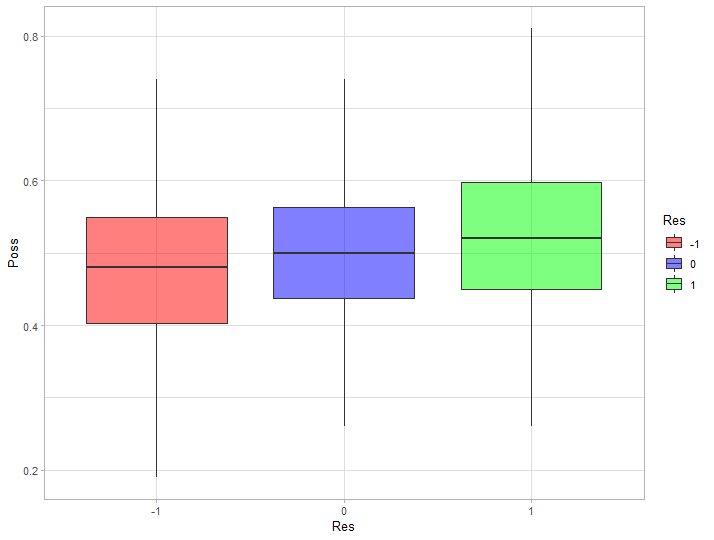
\includegraphics[scale=0.50]{Poss.png}
		\caption{Boxplot della distribuzione della variabile \texttt{Poss} rispetto ai valori della variabile risposta \texttt{Res}} \label{fig:Poss}
	\end{center}
\end{figure}
Nella Figura \ref{fig:sot} viene riportato il boxplot della distribuzione della variabile \texttt{SoT} rispetto ai valori della variabile risposta \texttt{Res}. Valori più alti sono presenti nella vittoria mentre valori molto più bassi sono presenti nella sconfitta. C'è una buona distribuzione dei valori nella vittoria dato che i baffi sono simmetrici, viceversa per gli altri due boxplot non c'è simmetria, infatti, il baffo inferiore è molto più corto rispetto al baffo superiore, segno che la maggior parte dei valori sono bassi e simili tra loro. Inoltre, alcuni outliers si discostano dalla distribuzione di tutti e tre i boxplot, questo perché ci sono state squadre che hanno tirato molte volte in porta. Le mediane dei boxplot pareggio e vittoria non sono equidistanti dai quantili ma più vicine al 1$^{\circ}$ quantile. Il boxplot della sconfitta ha una bassa varianza. In conclusione, avere un valore alto di tiri in porta sembra essere utile ai fini della vittoria.\\
Per la relazione tra la variabile risposta \texttt{Res} e la variabile \texttt{Sh}, si ha un boxplot molto simile al boxplot mostrato nella Figura \ref{fig:Poss}. Il grafico di \texttt{Sh} rispetto al grafico di \texttt{Poss} ha degli outliers e la mediana della sconfitta non è equidistante dai quantili ma più vicina al 1$^{\circ}$ quantile.\\
\begin{figure}[htbp]
	\begin{center}
		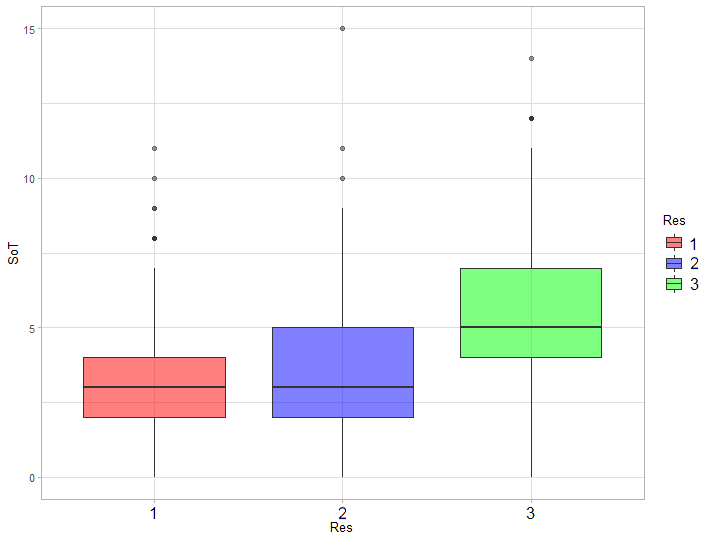
\includegraphics[scale=0.50]{SoT.png}
		\caption{Boxplot della distribuzione della variabile \texttt{SoT} rispetto ai valori della variabile risposta \texttt{Res} } \label{fig:sot}
	\end{center}
\end{figure}
Nella Figura \ref{fig:g} viene riportato il boxplot della distribuzione della variabile \texttt{G/Sh} rispetto ai valori della variabile risposta \texttt{Res}. Si nota che ci sono valori molto bassi ma leggermente più alti per la vittoria. La distribuzione non è buona perché i baffi sono asimmetrici, infatti, tutti i valori sono concentrati in basso e pochi verso il baffo superiore, segno che la maggior parte dei valori sono bassi e simili tra loro. C'è una bassa varianza tra i valori e la presenza di outliers perché alcune squadre sono riuscite a ottenere il massimo da ogni tiro. I risultati mostrati, nonostante la distribuzione, sono comunque coerenti dato che non ci si aspetta dal rapporto tiri-gol un numero alto ma comunque una tendenza che favorisca la vittoria.\\
\begin{figure}[htbp]
	\begin{center}
		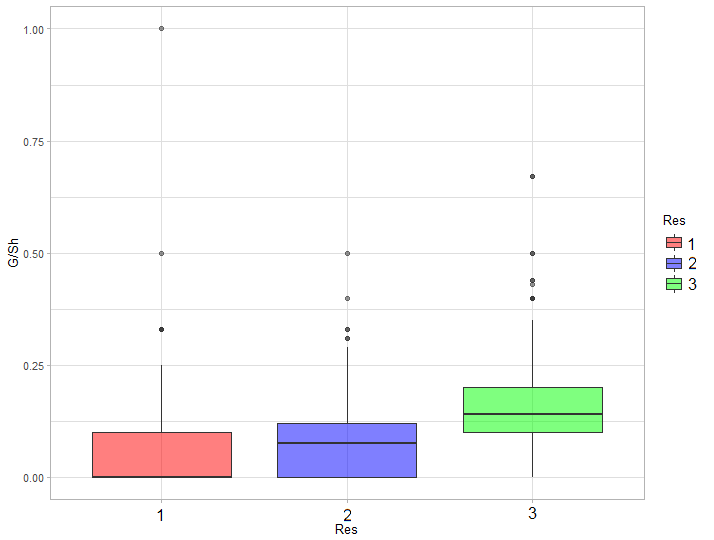
\includegraphics[scale=0.50]{g.png}
		\caption{Boxplot della distribuzione della variabile \texttt{G/Sh} rispetto ai valori della variabile risposta \texttt{Res} } \label{fig:g}
	\end{center}
\end{figure}
Nella Figura \ref{fig:saves} viene riportato il boxplot della distribuzione della variabile \texttt{Saves} rispetto ai valori della variabile risposta \texttt{Res}. Come si può notare sembra che \texttt{Saves} sia poco significativa ai fini del risultato. Infatti, c'è poca variazione tra un boxplot e l'altro perché sembra che avere un alto numero di parate non è determinante a fini del risultato.\\
\begin{figure}[htbp]
	\begin{center}
		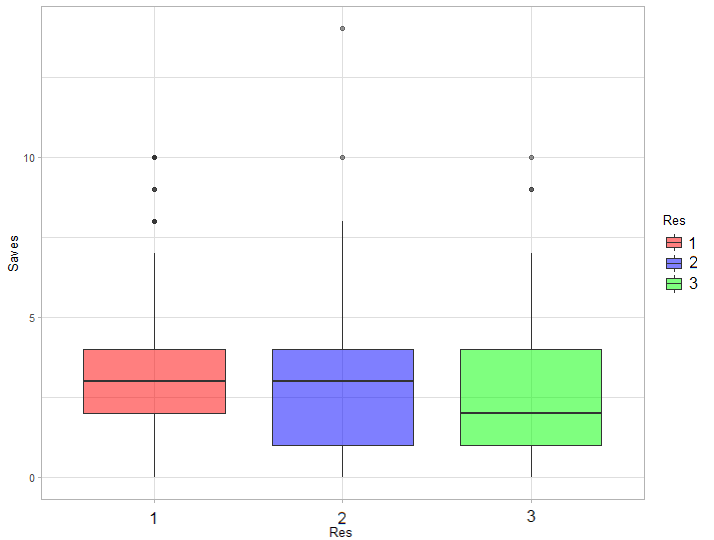
\includegraphics[scale=0.50]{saves.png}
		\caption{Boxplot della distribuzione della variabile \texttt{Saves} rispetto ai valori della variabile risposta \texttt{Res} } \label{fig:saves}
	\end{center}
\end{figure}
La Figura \ref{fig:pass} viene riportato a sinistra il boxplot della variabile numerica \texttt{PAtt} rispetto ai valori della variabile risposta \texttt{Res} e a destra il boxplot della variabile numerica \texttt{PCmp\%} rispetto ai valori della variabile risposta \texttt{Res}. Per entrambi sembra significativo l'elevato numero di passaggi tentati ma soprattutto quelli completati ai fini della vittoria. Nel grafico a sinistra, nel secondo e terzo boxplot il baffo superiore è più lungo rispetto al baffo inferiore, segno che molti valori sono bassi e simili tra loro, viceversa il primo boxplot ha una buona distribuzione perché i baffi sono simmetrici. Il boxplot della vittoria ha una maggiore varianza rispetto agli altri due e in più ha valori più alti; sia la mediana del boxplot della vittoria e sia quella del pareggio sono più vicine al 1$^{\circ}$ quantile, viceversa quella della sconfitta. I dati nel primo boxplot sembrano essere coerenti con l'esito della partita perché, maggiore è numero di passaggi che si prova ad effettuare, maggiori sono le possibilità di vittoria. Occorre però sapere quanto è precisa la squadra e questo lo si può scoprire con la variabile \texttt{PCmp\%}\\
Nel grafico a destra, si notano valori alti e molti outliers con valori bassi dovuti al fatto che ci sono state partite dove alcune squadre sono state poco precise nei passaggi. I baffi superiori di tutti e tre i boxplot sono molto meno lunghi rispetto ai baffi inferiori segno che molti valori sono alti e simili tra loro, inoltre, le varianze dei box sembrano essere uguali tra di loro. Sorprendentemente l'andamento invece di essere sempre crescente, prima scende da sconfitta a pareggio e poi sale da pareggio a vittoria.\\
Per la relazione tra la variabile risposta e la variabile \texttt{SPAtt}, si ha un grafico molto simile al grafico a sinistra della Figura \ref{fig:pass}. Il grafico di \texttt{SPAtt} rispetto al grafico di \texttt{PAtt} ha un maggior numero di outliers soprattutto per la sconfitta rispetto al grafico \texttt{PAtt} inoltre, c'è una minor varianza per tutti i tre boxplot oltre a valori più bassi in generale, questo è naturale perché \texttt{PAtt} contiene tutti i passaggi tentati e non solo quelli corti.\\
Per la relazione tra la variabile risposta e la variabile \texttt{SPCmp\%}, si ha un grafico molto simile al grafico a destra della Figura \ref{fig:pass}. Nel grafico di \texttt{SPCmp\%} rispetto al grafico di \texttt{PCmp\%}, il boxplot della sconfitta ha una maggior varianza, viceversa per la vittoria, che ha una minor varianza.\\
Per la relazione tra la variabile risposta \texttt{Res} e la variabile \texttt{MPAtt}, si ha un grafico molto simile al grafico a sinistra della Figura \ref{fig:pass}. Nel grafico di \texttt{MPAtt} rispetto al grafico di \texttt{PAtt}, il boxplot della sconfitta ha una maggior varianza. In generale i valori sono più bassi rispetto al grafico di \texttt{PAtt} ma questo è naturale perché \texttt{PAtt} contiene tutti i passaggi tentati e non solo quelli medi.\\
Per la relazione tra la variabile risposta e la variabile \texttt{MPCmp\%}, si ha un grafico molto simile al grafico a destra della Figura \ref{fig:pass}. Il grafico di \texttt{MPCmp\%} rispetto al grafico di \texttt{PCmp\%} ha valori più alti e molti più outliers inoltre, i baffi inferiore dei boxplot della sconfitta e della vittoria sono più corti.\\
Per la relazione tra la variabile risposta e la variabile \texttt{LPAtt}, si ha un grafico molto simile al grafico a sinistra della Figura \ref{fig:pass}. Nel grafico di \texttt{LPAtt} rispetto al grafico di \texttt{PAtt}, il boxplot della sconfitta ha valori più bassi rispetto agli boxplot del pareggio e della vittoria inoltre, il boxplot del pareggio ha una maggior varianza dei valori mentre il boxplot della vittoria ha una minor varianza. In generale i valori sono più bassi rispetto al grafico di \texttt{PAtt} ma questo è naturale perché \texttt{PAtt} contiene tutti i passaggi tentati e non solo quelli lunghi.\\
Per la relazione tra la variabile risposta e la variabile \texttt{LPCmp\%}, si ha un grafico molto simile al grafico a destra della Figura \ref{fig:pass}. Il grafico di \texttt{LPCmp\%} rispetto al grafico di \texttt{PCmp\%} ha valori più bassi, la distribuzione dei valori per il boxplot della sconfitta è ben equilibrata perché i baffi sono della stessa lunghezza e in più la mediana è equidistante dai due quantili. Analogamente anche il boxplot del pareggio ha una distribuzione equilibrata ma con più varianza e con una mediana equidistante dai quantili.\\
\begin{figure}[htbp]
	\begin{center}
		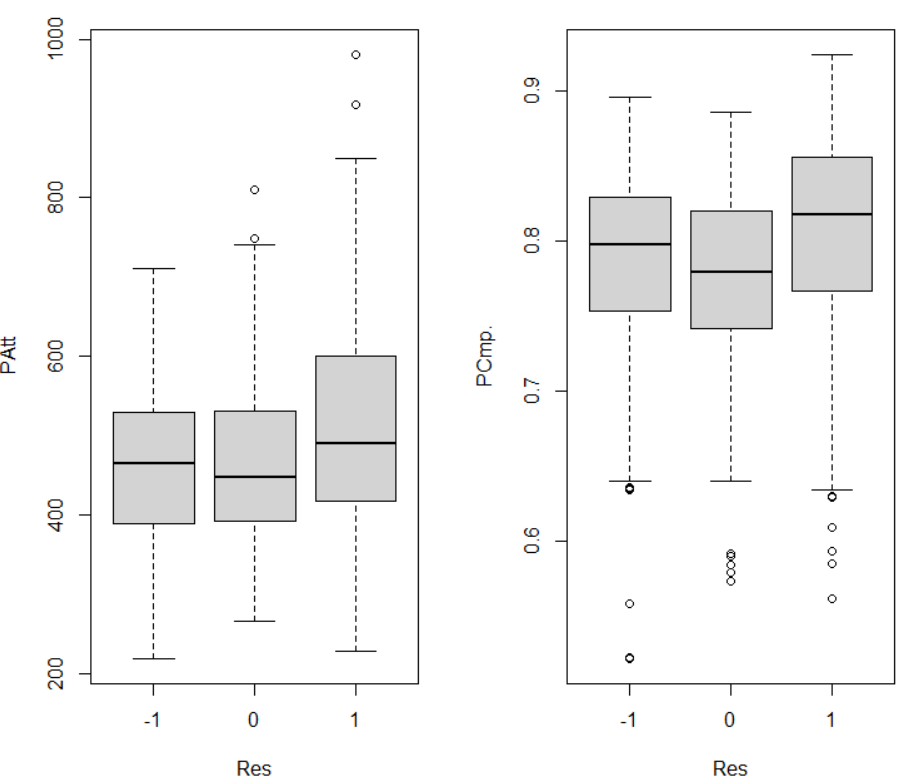
\includegraphics[height=8cm,width=13cm]{pass.png}
		\caption{A sinistra il boxplot della variabile numerica \texttt{PAtt} rispetto ai valori della variabile risposta \texttt{Res} e a destra il boxplot della variabile numerica \texttt{PCmp\%} rispetto ai valori della variabile risposta \texttt{Res}} \label{fig:pass}
	\end{center}
\end{figure}
Nella Figura \ref{fig:defp} viene riportato il boxplot della distribuzione della variabile \texttt{ToDefPen} rispetto ai valori della variabile risposta \texttt{Res}. Da ciò si può ipotizzare che \texttt{ToDefPen} non è significativa per la variabile risposta. Prima di escluderla si andrà ad analizzare se c'è qualche interazione con altre variabili che la fanno diventare significativa.\\
\begin{figure}[htbp]
	\begin{center}
		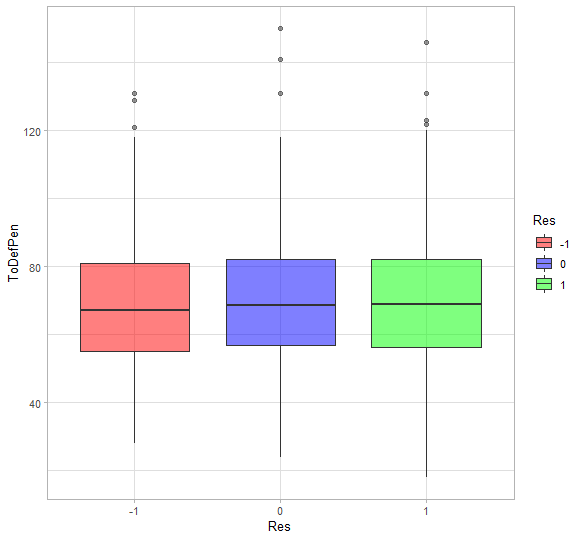
\includegraphics[scale=0.50]{def.png}
		\caption{Boxplot della distribuzione della variabile \texttt{ToDefPen} rispetto ai valori della variabile risposta \texttt{Res} } \label{fig:defp}
	\end{center}
\end{figure}
Nella Figura \ref{fig:att} viene riportato il boxplot della distribuzione della variabile \texttt{ToAttPen} rispetto ai valori della variabile risposta \texttt{Res}. Contrariamente quanto visto con la Figura \ref{fig:defp} qui si nota una certa variazione tra i boxplot infatti, i valori crescono dal boxplot della sconfitta fino al boxplot della vittoria. C'è una maggior varianza per il boxplot della vittoria rispetto agli altri due boxplot. Per tutti e tre i boxplot i baffi inferiori sono leggermente meno lunghi rispetto ai baffi superiori, segno che i valori sono bassi e simili tra loro, infatti, ci sono alcuni outliers sopra al baffo superiore, segno che alcune squadre in qualche partita si sono particolarmente rese note nel produrre un quantitativo di tocchi maggiore rispetto alla distribuzione, ciò però non sembra influenzare l'esito. Le mediane sono equidistanti.\\
Per la relazione tra la variabile risposta e la variabile \texttt{ToDef3rd}, si ha un grafico molto simile a quello mostrato nella Figura \ref{fig:att}. Il grafico di \texttt{ToDef3rd} rispetto al grafico di \texttt{ToAttPen} ha un minore numero di outliers soprattutto per il boxplot del pareggio, tale boxplot ha inoltre una varianza simile al boxplot della sconfitta. Il boxplot della vittoria invece, ha una distribuzione ben equilibrata.\\
Per la relazione tra la variabile risposta e la variabile \texttt{ToMid3rd}, si ha un grafico molto simile a quello mostrato nella Figura \ref{fig:att}. Il grafico di \texttt{ToMid3rd} rispetto al grafico di \texttt{ToAttPen} ha un minore numero di outliers e la varianza del boxplot della sconfitta è molto simile alla mediana del boxplot del pareggio ma con la mediana più vicina al 3$^{\circ}$ quantile.\\
Per la relazione tra la variabile risposta e la variabile \texttt{ToAtt3rd}, si ha un grafico molto simile a quello mostrato nella Figura \ref{fig:att}. Il grafico di \texttt{ToAtt3rd} rispetto al grafico di \texttt{ToAttPen} ha una minor varianza in generale per tutti e tre i boxplot e una distribuzione sbilanciata verso valori più bassi dato che tutti i baffi inferiori sono più corti rispetto ai baffi superiori. L'andamento però rimane lo stesso presente nella Figura \ref{fig:att}.\\
\begin{figure}[htbp]
	\begin{center}
		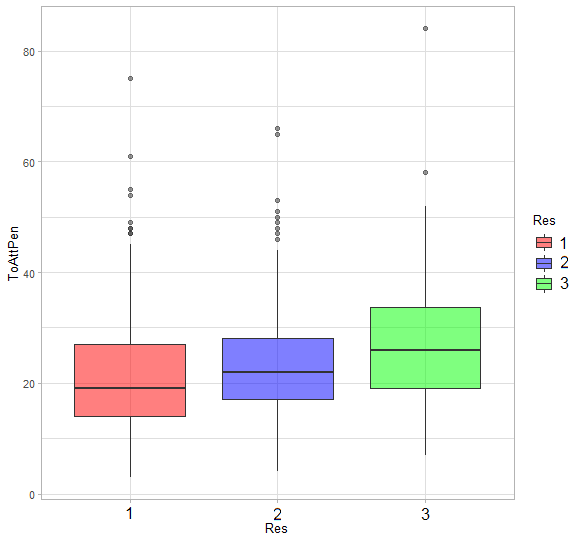
\includegraphics[scale=0.50]{att.png}
		\caption{Boxplot della distribuzione della variabile \texttt{ToAttPen} rispetto ai valori della variabile risposta \texttt{Res} } \label{fig:att}
	\end{center}
\end{figure}
Nella Figura \ref{fig:falli} vengono riportati a sinistra il boxplot della variabile numerica \texttt{Fls} rispetto ai valori della variabile risposta \texttt{Res} e a destra il boxplot della variabile numerica \texttt{Fld} rispetto ai valori della variabile risposta \texttt{Res}. Nel boxplot a sinistra si può notare che i valori più alti sono nel boxplot del pareggio e della vittoria ma nel boxplot del pareggio ci sono più valori alti in assoluto. Ciò fa ipotizzare che subire molti falli può impedire la vittoria alla squadra che li subisce. Per quanto riguarda la distribuzione sembra essere buona; c'è una minor varianza per quanto riguarda il boxplot della sconfitta. \\
\begin{figure}[htbp]
	\begin{center}
		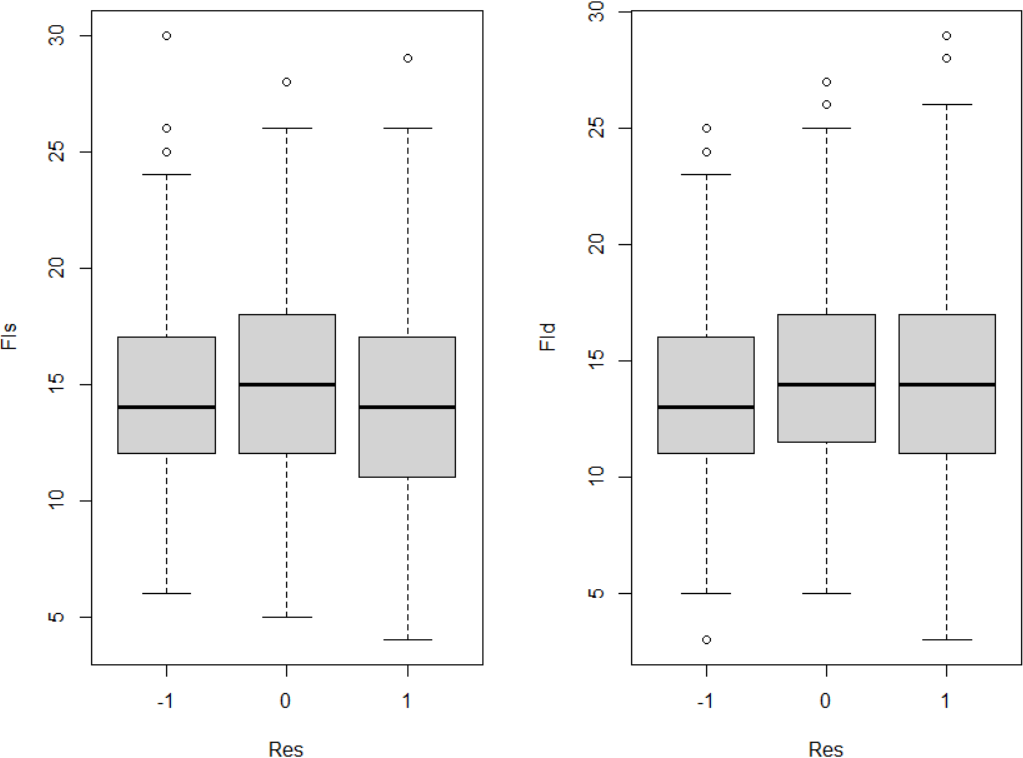
\includegraphics[height=8cm,width=13cm]{falli.png}
		\caption{A sinistra il boxplot della variabile numerica \texttt{Fls} rispetto ai valori della variabile risposta \texttt{Res} e a destra il boxplot della variabile numerica \texttt{Fld} rispetto ai valori della variabile risposta \texttt{Res}} \label{fig:falli}
	\end{center}
\end{figure}
Nel secondo boxplot si hanno valori più alti nel boxplot della vittoria e una maggior varianza rispetto al boxplot della sconfitta. Sembra perciò che dal grafico si può intuire che se la squadra non commette dei falli allora sarà più soggetta a perdere.\\
Per la relazione tra la variabile risposta \texttt{Res} e la variabile \texttt{Off}, si ha un grafico molto simile a quello mostrato nella Figura \ref{fig:saves}. Il grafico di \texttt{Off} rispetto al grafico di \texttt{Saves} ha un numero minore di valori per il boxplot della sconfitta rispetto agli altri due boxplot inoltre, le mediane del boxplot della sconfitta e del pareggio sono attaccate al 1$^{\circ}$ quantile.\\
Per la relazione tra la variabile risposta \texttt{Res} e la variabile \texttt{Crs}, si ha un grafico molto simile a quello mostrato nella Figura \ref{fig:int}. Nel grafico di \texttt{Crs} rispetto al grafico di \texttt{Saves}, il boxplot della sconfitta ha maggior varianza e il baffo inferiore dei boxplot della sconfitta e della vittoria sono più corti rispetto ai baffi superiori.\\
Nella Figura \ref{fig:int} viene riportato il boxplot della distribuzione della variabile \texttt{Int} rispetto ai valori della variabile risposta \texttt{Res}. Sorprendentemente, valori più alti sono registrati nel boxplot della sconfitta, anche se la mediana risulta essere più vicina al 1$^{\circ}$ quantile sottolineando che c'è un maggior numero di valori bassi piuttosto che alti. Le mediane dei restanti boxplot invece, sono ben equilibrate ma il boxplot del pareggio risulta avere meno varianza. Sembra perciò che effettuare troppe intercettazioni dei passaggi avversari contrariamente da quanto si pensi sia controproducente per la vittoria. Si segnala inoltre la presenza di alcuni outliers con valori alti di intercettazioni che si discostano dalle distribuzioni.\\
\begin{figure}[htbp]
	\begin{center}
		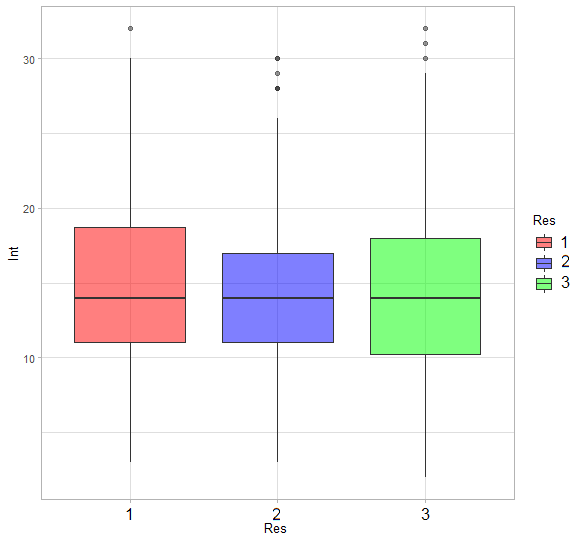
\includegraphics[scale=0.50]{int.png}
		\caption{Boxplot della distribuzione della variabile \texttt{Int} rispetto ai valori della variabile risposta \texttt{Res}} \label{fig:int}
	\end{center}
\end{figure}
Nella Figura \ref{fig:tkl} viene riportato il boxplot della distribuzione della variabile \texttt{TklWin} rispetto ai valori della variabile risposta \texttt{Res}. Come si può notare, vincere più contrasti possibili evita di subire una sconfitta. Infatti, ci sono valori più alti nei boxplot del pareggio e della vittoria rispetto al boxplot della sconfitta. Nello specifico però si nota che: nella distribuzione c'è una maggior presenza di valori alti nella vittoria rispetto al pareggio, graficamente lo si vede dalla mediana che nel boxplot del pareggio è più vicina al 1$^{\circ}$ quindi ha valori più bassi e lo si nota anche dal baffo inferiore che è meno lungo rispetto a quello superiore viceversa. La mediana del boxplot della vittoria risulta più vicina al 3$^{\circ}$ oltre ad avere il baffo superiore più corto rispetto a quello inferiore. C'è inoltre qualche outliers con valori più alti di contrasti vinti ma sembrano non influenzare la classificazione.\\
\begin{figure}[htbp]
	\begin{center}
		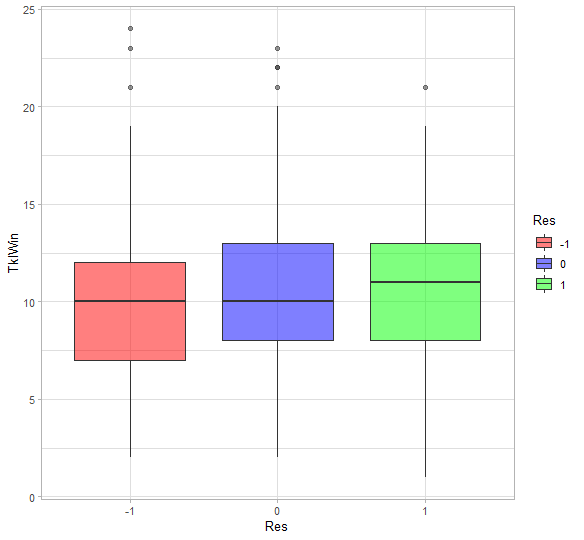
\includegraphics[scale=0.50]{tklwin.png}
		\caption{Boxplot della distribuzione della variabile \texttt{TklWin} rispetto ai valori della variabile risposta \texttt{Res}} \label{fig:tkl}
	\end{center}
\end{figure}
\begin{figure}[htbp]
	\begin{center}
		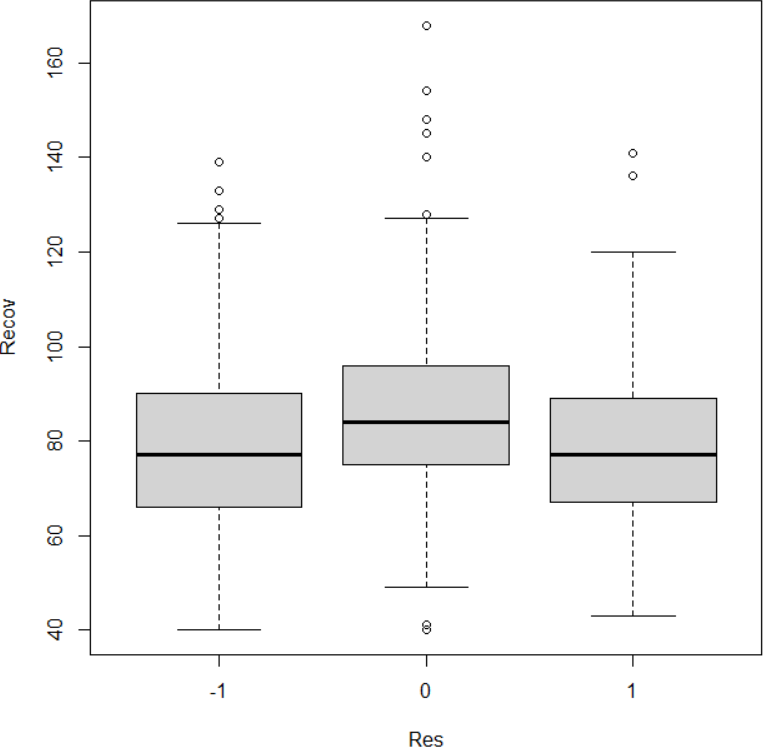
\includegraphics[scale=0.50]{recov.png}
		\caption{Boxplot della distribuzione della variabile \texttt{Recov} rispetto ai valori della variabile risposta \texttt{Res}} \label{fig:recov}
	\end{center}
\end{figure} 
Infine nella Figura \ref{fig:recov} viene riportato il boxplot della distribuzione della variabile \texttt{Recov} rispetto ai valori della variabile risposta \texttt{Res}. Per entrambi i boxplot la distribuzione sembra più sbilanciata verso valori bassi quindi ad una loro maggior presenza. Infatti, entrambi i baffi inferiori sono più corti rispetto a quelle superiori. Per quanto riguarda la mediana sembra equidistante dai quantili per entrambi i tre boxplot. Si nota che il boxplot del pareggio presenta minor varianza rispetto agli altri due boxplot ma valori più alti soprattutto nei confronti del boxplot della vittoria. Perciò, un eccessivo numero di recuperi non porti alla vittoria. Inoltre, ci sono numerosi outliers.

\subsection{Analisi possibili interazioni} 
Per concludere l'attività di preprossening, non resta che analizzare le relazioni tra le covariate per individuare possibili interazioni tra di loro che possono influenzare la variabile risposta. Chiaramente dato che ci sono più di trenta variabili e dunque, un grandissimo numero di combinazioni, non si sono esaminate tutte le relazioni ma sono state selezionate solo alcune per l'analisi, basandosi su teorie calcistiche esaminate durante la fase di studio del problema.\\
Per l'analisi delle interazioni si sono utilizzati i grafici di dispersione. Un grafico di dispersione mostra la relazione tra due variabili continue. A tali grafici si è inserito una terza variabile, la variabile risposta \texttt{Res}, dove ogni punto è colorato in tre possibili colori che rappresentano una delle tre categorie di \texttt{Res}. Di conseguenza il grafico permette di visualizzare se le categorie sono ben separate e quindi se un'interazione può spiegare l'andamento dei punti della variabile risposta.\\
Inoltre, è stato utilizzato l'indice di correlazione, che indica la forza dell'associazione lineare espressa in valori compresi tra -1 e 1. Tale misura permette di escludere da subito alcune relazioni tra variabili se l'indice è troppo alto o basso, infatti, le relazioni troppo forti vanno escluse perché possono generare il fenomeno della collinearità. La collinearità è quel fenomeno che va a nasconde il legame tra le variabili e la variabile risposta, a causa di un legame troppo forte tra le covariate.\\
Nella Figura \ref{fig:cor} viene mostrato il valore della correlazione per ogni possibile relazione tra variabili numeriche. Si nota che ci sono molte relazioni che hanno un valore di correlazione molto vicino a 1, in basso a sinistra del grafico. Ad esempio notiamo che la variabile \texttt{SPCmp\%} ha una relazione molto forte con la variabile \texttt{PCmp\%} (correlazione = 0.82), ciò è coerente perché, la variabile \texttt{SPCmp\%} contiene solo i passaggi corti completati mentre \texttt{PCmp\%} contiene tutti i tipi di passaggi completati, ne consegue che la ridondanza dei dati causa questa alta correlazione. Analogamente la stessa motivazione la si può applicare tra la variabile \texttt{PAtt} e la variabile \texttt{SPAtt} (correlazione = 0.91). Perciò tale motivazione è applicabile a tutte le variabili relative ai passaggi completati o relative ai passaggi tentati.
\begin{figure}[htbp]
	\begin{center}
		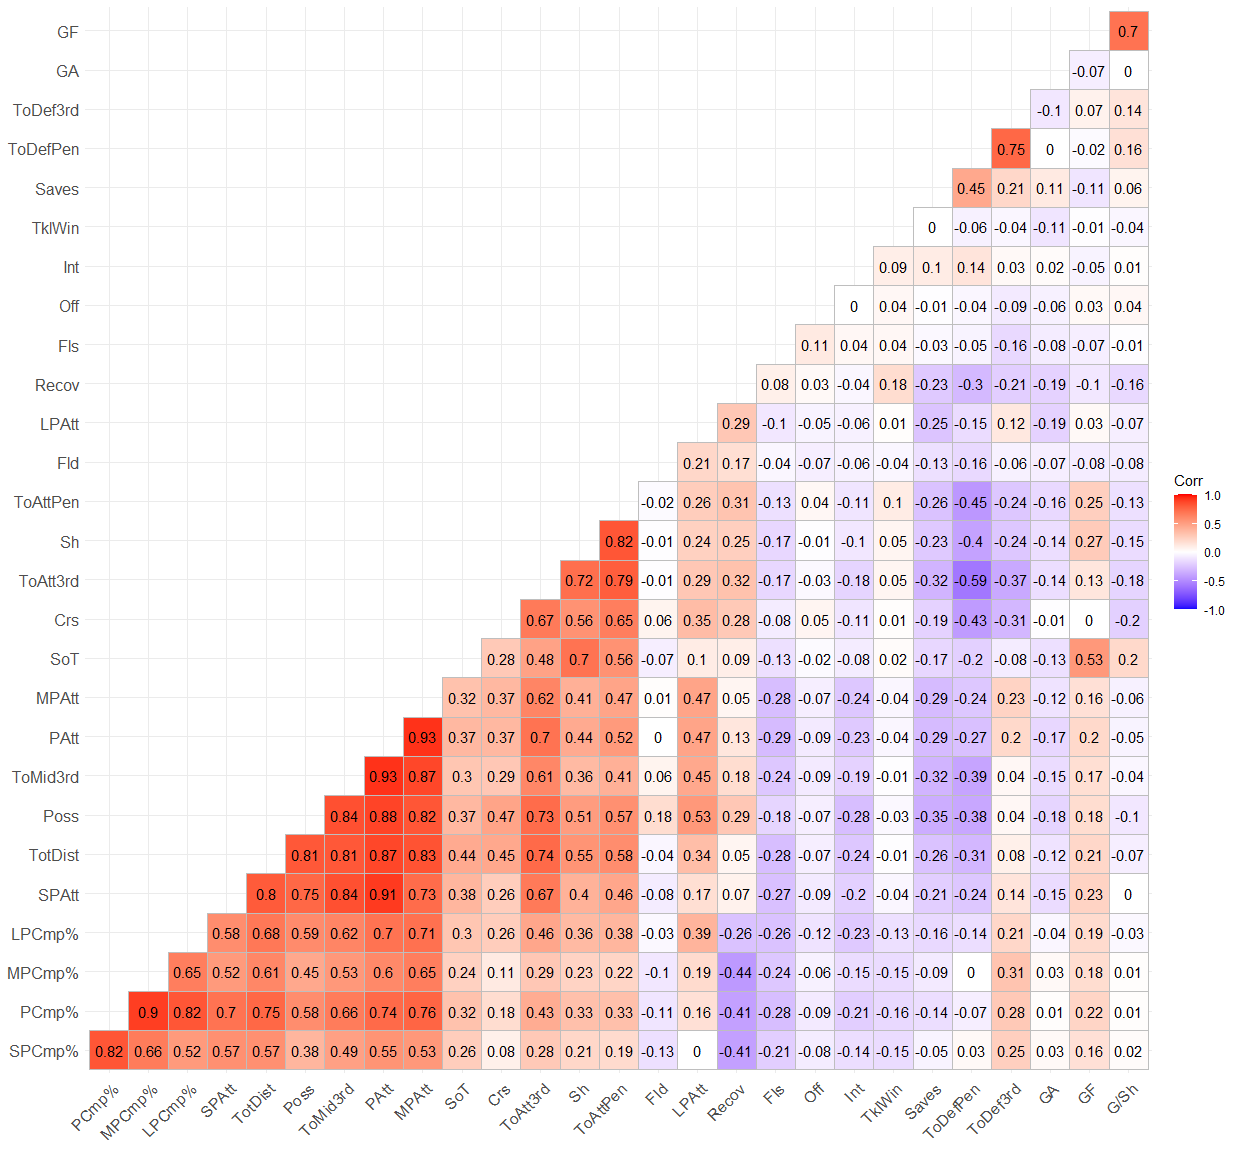
\includegraphics[scale=0.47]{Rplot.png}
		\caption{Grafico delle correlazioni di ogni coppia di variabili}  \label{fig:cor}
	\end{center}
\end{figure}
Di seguito si riporteranno le interazioni che sono state individuate come significative.\\ 

Sono state individuate le seguenti tre interazioni con la variabile \texttt{Sh}:
\begin{itemize}
	\item Interazione tra la variabile \texttt{Sh} e la variabile \texttt{ToAttPen}. È ragionevole ipotizzare che il numero di tocchi fatti nell'area di rigore avversaria possano creare azioni da tiro. È quindi possibile che tra le due variabili possa esserci una relazione. La Figura \ref{fig:shpen} mostra una relazione positiva tra le due variabili infatti, quando aumenta la variabile \texttt{Sh} aumenta anche la variabile \texttt{ToAttPen} e viceversa. Sono distinguibili tre differenti gruppi che rappresentano le tre categorie della variabile risposta. Inoltre, la correlazione tra le due variabili non è troppo alta (0.72). Ne consegue che un'interazione tra la variabile \texttt{Sh} e la variabile \texttt{ToAttPen} sembra essere significativa rispetto alla variabile risposta.
	\begin{figure}[htbp]
		\begin{center}
			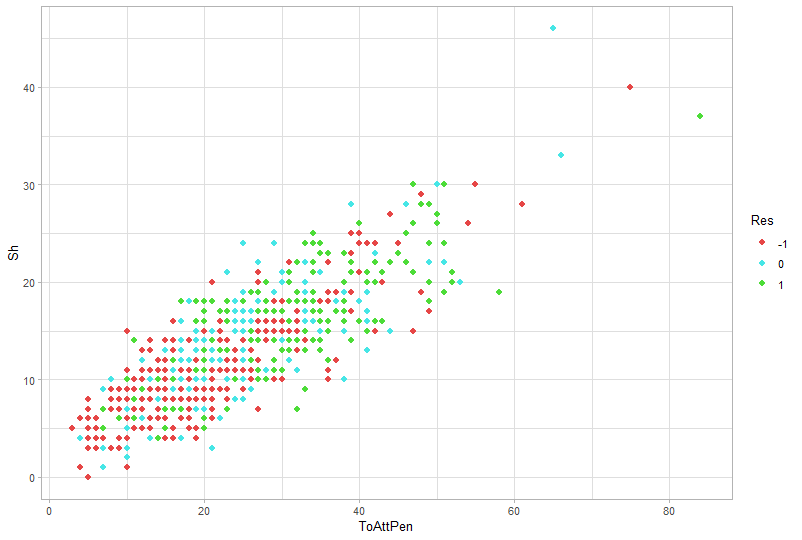
\includegraphics[scale=0.50]{sh-toattpen.png}
			\caption{Scatterplot della distribuzione della variabile \texttt{Sh} rispetto ai valori della variabile \texttt{ToAttPen}}  \label{fig:shpen}
		\end{center}
	\end{figure}
	\item Interazione tra la variabile \texttt{Sh} e la variabile \texttt{G/Sh}. È ragionevole ipotizzare che ci sia un legame naturale tra tiri fatti e rapporto tiri-gol. La Figura \ref{fig:shgol} mostra una relazione negativa tra le due variabili infatti, quando aumenta la variabile \texttt{Sh} diminuisce anche la variabile \texttt{G/Sh} e viceversa. Sono distinguibili tre differenti gruppi che rappresentano le tre categorie della variabile risposta infatti, i punti della categoria vittoria sono più in alto mentre i punti delle categorie pareggio e sconfitta più in basso. Inoltre, la correlazione tra le due variabili non è bassa (-0.15). Ne consegue che un'interazione tra la variabile \texttt{Sh} e la variabile \texttt{G/Sh} sembra essere significativa rispetto alla variabile risposta.
	\begin{figure}[htbp]
		\begin{center}
			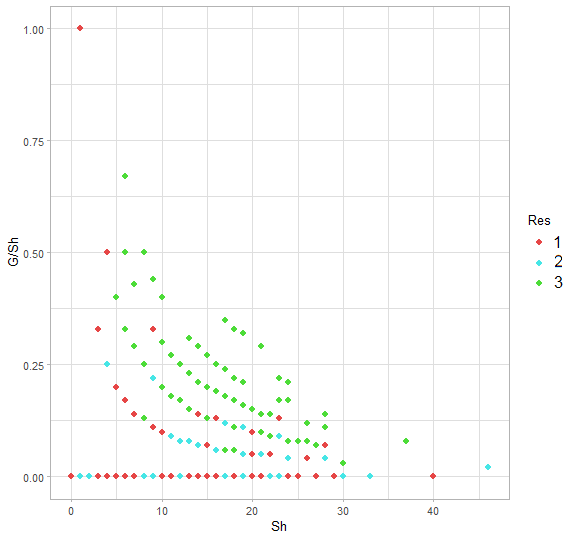
\includegraphics[scale=0.60]{sh-g.sh.png}
			\caption{Scatterplot della distribuzione della variabile \texttt{Sh} rispetto ai valori della variabile \texttt{G/Sh}}  \label{fig:shgol}
		\end{center}
	\end{figure}
	\item Interazione tra la variabile \texttt{Sh} e la variabile \texttt{Poss}. Generalmente è possibile ipotizzare che il possesso della palla possa favorire la squadra nell’effettuare i tiri. Infatti, la Figura \ref{fig:shposs} mostra una relazione positiva tra le due variabili, quando aumenta la variabile \texttt{Sh} aumenta anche la variabile \texttt{Poss} e viceversa. Sono distinguibili tre differenti gruppi che rappresentano le tre categorie della variabile risposta. Inizialmente i vari punti sono mescolati tra di loro ma, con l'avanzamento emergono le direzioni di ogni categoria infatti, i punti della categoria vittoria vanno più verso destra mentre i punti della categoria sconfitta si spostano verso l'alto. I punti della categoria pareggio invece, si muovono in mezzo ai punti delle altre due categorie. La correlazione tra le due variabili non è alta (0.51). Ne consegue che un'interazione tra la variabile \texttt{Sh} e la variabile \texttt{Poss} sembra essere significativa rispetto alla variabile risposta.
	\begin{figure}[htbp]
		\begin{center}
			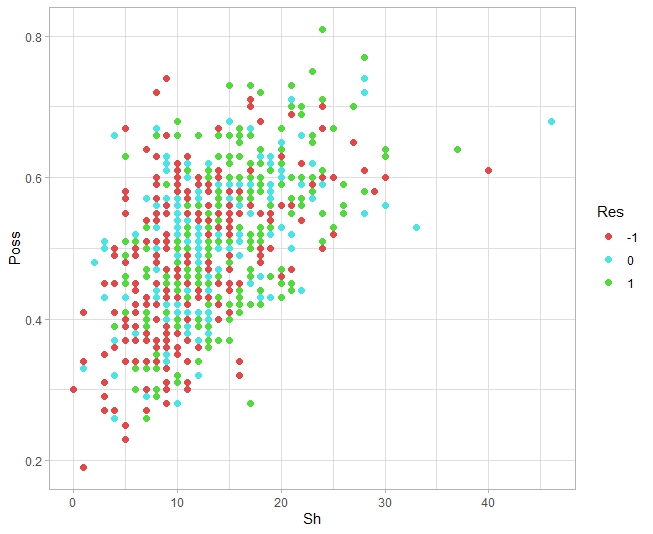
\includegraphics[scale=0.60]{poss-sh.png}
			\caption{Scatterplot della distribuzione della variabile \texttt{Sh} rispetto ai valori della variabile \texttt{Poss}}  \label{fig:shposs}
		\end{center}
	\end{figure}
\end{itemize}
Sono state individuate le seguenti tre interazioni con la variabile \texttt{ToMid3rd}:
\begin{itemize}
	\item Interazione tra la variabile \texttt{ToMid3rd} e la variabile \texttt{LPAtt}. Si suppone che tra le due variabili ci sia una relazione perché molti lanci lunghi per le punte partono proprio del centrocampo. La Figura \ref{fig:midl} mostra un andamento leggermente a "nuvola" ma comunque, è possibile individuare una relazione positiva tra le due variabili. Infatti, quando aumenta la variabile \texttt{ToMid3rd} aumenta anche la variabile \texttt{LPAtt} e viceversa. Sono distinguibili tre differenti gruppi che rappresentano le tre categorie della variabile risposta. Inizialmente i vari punti sono mescolati tra di loro ma, successivamente i punti della categoria vittoria vanno molto in alto mentre i punti della categoria sconfitta rimangono molto più bassi muovendosi verso destra, invece i punti della categoria pareggio anche essi vanno verso destra ma rimanendo più alti rispetto ai punti della categoria sconfitta. La correlazione tra le due variabili non è alta (0.45). Ne consegue che un'interazione tra la variabile \texttt{ToMid3rd} e la variabile \texttt{LPAtt} sembra essere significativa rispetto alla variabile risposta.
	\begin{figure}[htbp]
		\begin{center}
			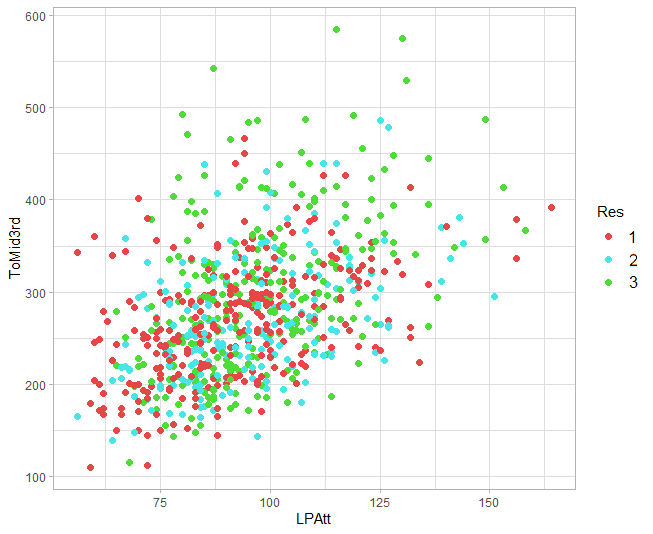
\includegraphics[scale=0.60]{mid-lpatt.png}
			\caption{Scatterplot della distribuzione della variabile \texttt{ToMid3rd} rispetto ai valori della variabile \texttt{LPAtt}}  \label{fig:midl}
		\end{center}
	\end{figure}
	\item Interazione tra la variabile \texttt{ToMid3rd} e la variabile \texttt{PCmp\%}. Per le stesse ragioni illustrate nel punto precedente si ipotizza una relazione tra le variabili. La Figura \ref{fig:midp} mostra una relazione positiva tra le due variabili infatti, quando aumenta la variabile \texttt{ToMid3rd} aumenta anche la variabile \texttt{PCmp\%} con un'andamento simile ad una funzione esponenziale. Sono distinguibili tre differenti gruppi che rappresentano le tre categorie della variabile risposta, dove i punti più in alto sono della categoria del pareggio, leggermente più sotto ci sono i punti della vittoria che però verso la fine del grafico raggiungono i valori più alti e infine, i punti della sconfitta. La correlazione tra le due variabili non è alta (0.66). Ne consegue che un'interazione tra la variabile \texttt{ToMid3rd} e la variabile \texttt{PCmp\%} sembra essere significativa rispetto alla variabile risposta.
	\begin{figure}[htbp]
		\begin{center}
			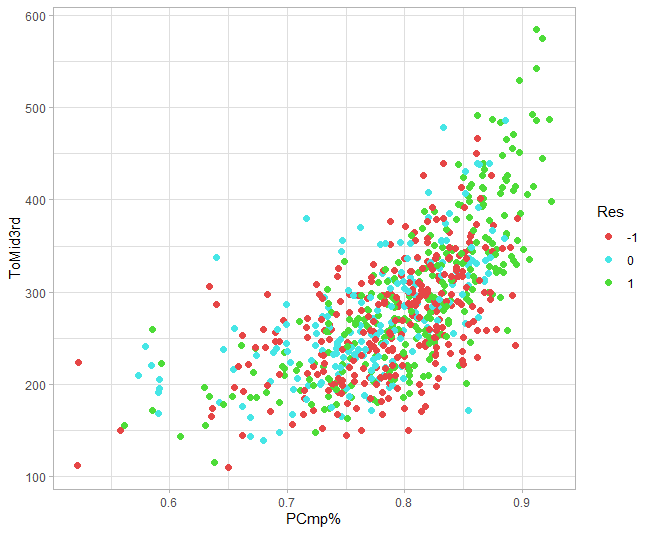
\includegraphics[scale=0.60]{mid-pcmp.png}
			\caption{Scatterplot della distribuzione della variabile \texttt{ToMid3rd} rispetto ai valori della variabile \texttt{PCmp\%}}  \label{fig:midp}
		\end{center}
	\end{figure}
\end{itemize}

Infine sono state individuate le seguenti interazioni:
\begin{itemize}
	\item Interazione tra la variabile \texttt{TotDist} e la variabile \texttt{PCmp\%}. Naturalmente per effettuare i passaggi e completarli è possibile farlo solo se ci si muove con la palla. La Figura \ref{fig:totdistpcmp} mostra una relazione positiva tra le due variabili infatti, quando aumenta la variabile \texttt{TotDist} aumenta anche la variabile \texttt{PCmp\%} con un'andamento simile ad una funzione esponenziale. Sono distinguibili tre differenti gruppi che rappresentano le tre categorie della variabile risposta, dove i punti più in alto sono della categoria del pareggio, leggermente più sotto ci sono i punti della vittoria e infine i punti della sconfitta. La correlazione tra le due variabili non è troppo alta (0.75). Ne consegue che un'interazione tra la variabile \texttt{TotDist} e la variabile \texttt{PCmp\%} sembra essere significativa rispetto alla variabile risposta.
	\begin{figure}[htbp]
		\begin{center}
			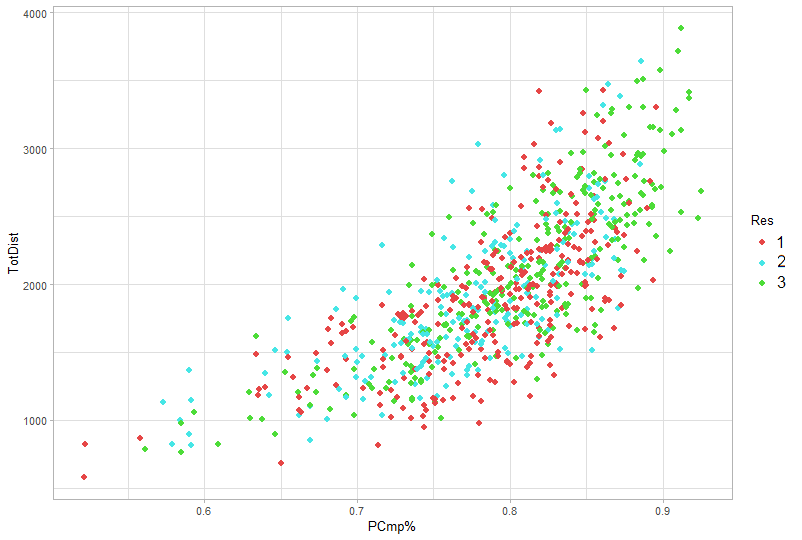
\includegraphics[scale=0.50]{TotDist-PCmp.png}
			\caption{Scatterplot della distribuzione della variabile \texttt{TotDist} rispetto ai valori della variabile\texttt{PCmp\%}}  \label{fig:totdistpcmp}
		\end{center}
	\end{figure}
	\item Interazione tra la variabile \texttt{PAtt} e la variabile \texttt{PCmp\%}. Data la loro naturale correlazione si ipotizza che ci sia un'interazione. La Figura \ref{fig:pp} mostra una relazione positiva tra le due variabili infatti, quando aumenta la variabile \texttt{PAtt} aumenta anche la variabile \texttt{PCmp\%} con un'andamento simile ad una funzione esponenziale. Sono distinguibili tre differenti gruppi che rappresentano le tre categorie della variabile risposta, dove i punti più in alto sono della categoria del pareggio, leggermente più sotto ci sono i punti della vittoria e infine i punti della sconfitta. La correlazione tra le due variabili non è troppo alta (0.74). Ne consegue che un'interazione tra la variabile \texttt{PAtt} e la variabile \texttt{PCmp\%} sembra essere significativa rispetto alla variabile risposta.
	\begin{figure}[htbp]
		\begin{center}
			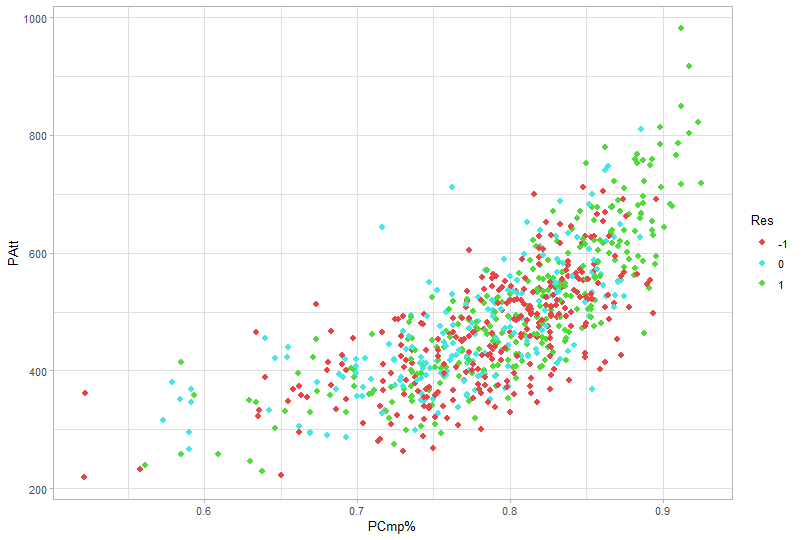
\includegraphics[scale=0.50]{PAtt-PCmp.png}
			\caption{Scatterplot della distribuzione della variabile \texttt{PAtt} rispetto ai valori della variabile \texttt{PCmp\%}}  \label{fig:pp}
		\end{center}
	\end{figure}
	\item Interazione tra la variabile \texttt{ToDefPen} e la variabile \texttt{ToAttPen}. Come ci si può aspettare la Figura \ref{fig:defatt} mostra una relazione negativa tra le due variabili, quando aumenta la variabile \texttt{ToDefPen} diminuisce anche la variabile \texttt{ToAttPen} e viceversa. Sono distinguibili tre differenti gruppi che rappresentano le tre categorie della variabile risposta infatti, i punti della categoria vittoria sono quelli più distanti dallo zero mentre i punti delle categorie pareggio e sconfitta sono più vicini allo zero. Inoltre, la correlazione tra le due variabili non è bassa (-0.45). Ne consegue che un'interazione tra la variabile \texttt{ToDefPen} e la variabile \texttt{ToAttPen} sembra essere significativa rispetto alla variabile risposta.
	\begin{figure}[htbp]
		\begin{center}
			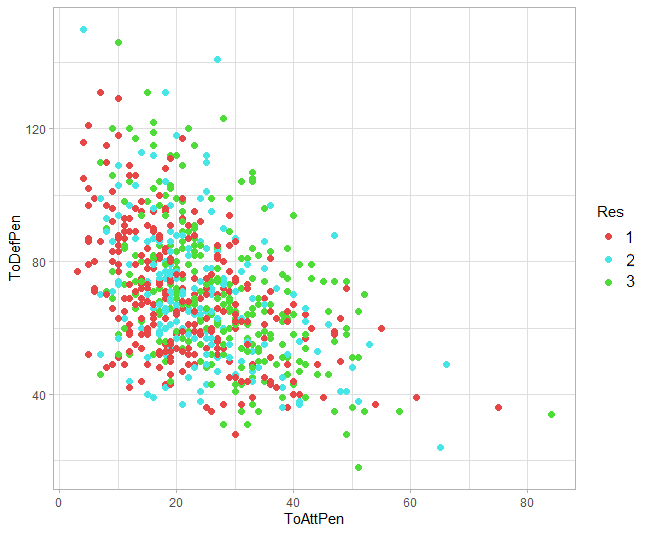
\includegraphics[scale=0.60]{def.att.png}
			\caption{Scatterplot della distribuzione della variabile \texttt{ToDefPen} rispetto ai valori della variabile \texttt{ToAttPen}}  \label{fig:defatt}
		\end{center}
	\end{figure}
	
\end{itemize}

\begin{comment}
	\subsection{Collinearità}
	Per collinearità si intende quel fenomeno per il quale se più variabili esplicative altamente correlate vengono inserite nel modello, allora la loro alta correlazione andrà a nasconde la loro associazione con la variabile risposta. La soluzione per risolvere questo problema è quella di scegliere soltanto una sola variabile della relazione da inserire nel modello.\\
	Nella Figura \ref{fig:cor} viene mostrato il valore della correlazione per ogni possibile interazione tra variabile numeriche.\\
	Come si può notare una maggior correlazione tra le variabili è concentra nella prima parte del triangolo. Dal grafico possiamo vedere come tutte le interazioni che sono state descritte nella sottosezione precedente abbiano un’alta correlazione ma non eccessivamente alta. Si hanno i seguenti valori di correlazione:
	\begin{itemize}
		\item Le interazioni con la variabile \texttt{Sh}:
		\begin{itemize}
			\item L'interazione tra \texttt{Sh} e \texttt{SoT} ha come valore 0,70 tale da giustificare l'inserimento dell'interazione.
			\item L'interazione tra \texttt{Sh} e \texttt{ToAtt3rd} ha come valore 0,72 tale da giustificare l'inserimento dell'interazione.
			\item L'interazione tra \texttt{Sh} e \texttt{ToAttPen} ha come valore 0,82 è un valore alto con un possibile rischio di collinearità. Tale valore però giustifica l'inserimento dell'interazione.
		\end{itemize}
		\item Le interazioni con la variabile \texttt{Poss}:
		\begin{itemize}
			\item L'interazione tra \texttt{Poss} e \texttt{PAtt} ha come valore 0,88 è un valore molto alto con un possibile rischio di collinearità. Tale valore però giustifica l'inserimento dell'interazione.
			\item L'interazione tra \texttt{Poss} e \texttt{PAtt} ha come valore 0,81 è un valore alto con un possibile rischio di collinearità. Tale valore però giustifica l'inserimento dell'interazione.
		\end{itemize}
		\item Le interazioni con la variabile \texttt{TotDist}:
		\begin{itemize}
			\item L'interazione tra \texttt{TotDist} e \texttt{PAtt} ha come valore 0,87 è un valore molto alto con un possibile rischio di collinearità. Tale valore però giustifica l'inserimento dell'interazione.
			\item L'interazione tra \texttt{TotDist} e \texttt{PCmp\%} ha come valore 0,75 tale da giustificare l'inserimento dell'interazione.
		\end{itemize}
		
		\item L'interazione tra \texttt{ToAtt3rd} e \texttt{PAttPen} ha come valore 0,79 tale da giustificare l'inserimento dell'interazione.
		\item L'interazione tra \texttt{PAtt} e \texttt{PCmp\%} ha come valore 0,74 tale da giustificare l'inserimento dell'interazione.
	\end{itemize}  
	
	
	Nella sottosezione precedente si poteva pensare di inserire interazioni abbastanza naturali ad esempio: \texttt{PAtt}*\texttt{SPAtt}, \texttt{PAtt}*\texttt{MPAtt} e, \texttt{PCmp\%}*\texttt{MPCmp\%} e \texttt{PAtt}*\texttt{LPCmp\%}. Tali interazioni però sono composte da variabili che hanno un’alta correlazione tra loro, e quindi si ha il rischio di incombere in un problema di collinearità. Una correlazione cos^ alta era prevedibile dato che c'è una ridondanza dei dati tra le variabili. In questa fase dell'analisi non si hanno abbastanza elementi per poter scegliere quale variabile tenere e quale no, perciò, tale scelta verrà rinviata alla fase di modellazione.\\
	Il grafico suggerisce alcune interazioni che non sono state descritti ad esempio:\\ \texttt{Poss}*\texttt{ToAtt3rd}, \texttt{Poss}*\texttt{SPAtt},  \texttt{TotDist}*\texttt{ToAtt3rd}, \texttt{PCmp\%}*\texttt{SPAtt} e \texttt{PCmp\%}*\texttt{MPAtt}.
	Tali interazioni saranno analizzate durante la fase di modellazione per verificare se effettivamente sono significative per il modello.\\
	Infine si nota una buona correlazione tra \texttt{ToDefPen} e \texttt{ToDef3rd}, l'interazione può essere inserita perché va a giustificare il fatto che la variabile \texttt{ToDefPen} combinata con \texttt{ToDef3rd} diventa significativa per la variabile risposta....
\end{comment}




%\begin{figure}[htbp]
%	\begin{center}
	%		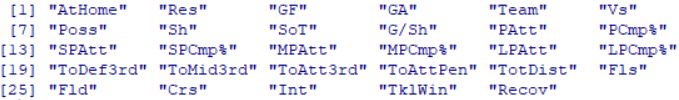
\includegraphics[scale=0.70]{cov.png}
	%		\caption{Grafico riassuntivo delle variabili rimaste dopo il Prepossesing}  \label{fig:cov}
	%	\end{center}
%\end{figure}
\begin{comment}
	
	
	\section{Ulteriori modifiche del dataset}
	
	Nelle sezioni precedenti si è descritto come si è costruito il dataset e come esso è stato strutturato. Tale struttura ha il vantaggio di rendere il dataset di facile interpretazione, ma deve essere riadattato per poter utilizzare le funzioni del pacchetto \texttt{BradleyTerry2}.\\ 
	Sono state apportare le seguenti modifiche.\\
	
	Innanzitutto il modello richiede che le due variabili \texttt{Team} e \texttt{Vs} siano di tipo fattore oppure costituiscano un \textsf{data.frame}. Un \textsf{data.frame} è una raccolta di vettori di osservazioni, che devono avere tutti la stessa lunghezza, ma possono essere di tipo diverso: variabili nominali (fattori) o variabili numeriche.
	Le variabili \textsf{Team} e \textsf{Vs} sono state trasformate in \texttt{data.frame} in modo da poter inserire al loro interno tutte le covariate descritte nella sezione precedente.
	
	Inoltre i valori della variabile \texttt{AtHome} sono stati converti in 1 (se \texttt{TRUE}) mentre in 0 (se \texttt{FALSE}).
	
\end{comment}
\pagebreak
\section{Ulteriori modifiche del dataset}

Nelle sezioni precedenti si è descritto come si è costruito il \emph{dataset} e come esso è stato strutturato. Tale struttura ha il vantaggio di rendere il \emph{dataset} di facile interpretazione, ma deve essere riadattato per poter utilizzare le funzioni del pacchetto \textit{\cite{bt2}} e del pacchetto \textit{\cite{btl}}.\\ 
Di seguito vengono presentate le modifiche effettuate specifiche per i due pacchetti.
\subsection{Modifiche per il pacchetto BradleyTerry2}
Innanzitutto il modello richiede che le due variabili \texttt{Team} e \texttt{Vs} siano di tipo fattore oppure che costituiscano un \textsf{data.frame}. Un \textsf{data.frame} è una raccolta di vettori di osservazioni che devono avere tutti la stessa lunghezza ma possono essere di tipo diverso: variabili nominali (fattori) o variabili numeriche.
Le variabili \textsf{Team} e \textsf{Vs} sono state trasformate in \texttt{data.frame} in modo da poter inserire al loro interno tutte le variabili descritte nella sezione precedente. Inoltre, i valori della variabile \texttt{AtHome} sono stati converti in 1 se \texttt{TRUE} mentre in 0 se \texttt{FALSE}.\\
Per poter creare i due \texttt{data.frame} occorre raccogliere le informazioni sulle partite giocate fuori casa dalle squadre indicate nella variabile \texttt{Team}. Con la funzione \ref{code:a1} viene implementato ciò in R. La definizione è la seguente.\\
Innanzitutto viene creato un vettore vuoto per ogni variabile presente nel \emph{dataset}, ad eccezione di \textsf{AtHome} che verrà gestita in un modo diverso. Viene creato il vettore \texttt{del} che tiene traccia di quali osservazioni saranno da eliminare. Si eliminano le osservazioni delle partite giocate fuori casa dalle squadre indicate nella variabile \texttt{Team} perché dopo le modifiche saranno ridondanti. La variabile \texttt{k} è l'indice usato per scorre il \emph{dataset} per trovare i dati dell'avversario. La variabile \texttt{z} è l'indice usato per inserire un nuovo elemento nel vettore \texttt{del}. Il funzionamento è il seguente.\\
Il primo ciclo \texttt{for} scorre tutto il \emph{dataset} alla ricerca delle righe con i dati delle partite giocate in casa dalla squadra indicata in \texttt{Team} infatti, al suo interno il primo costrutto \texttt{if} controlla se la partita è in casa per \texttt{Team} se sì, parte un secondo ciclo \texttt{for} che anche esso scorre tutto il \emph{dataset} per cercare la riga con la partita giocata della squadra indicata in \texttt{Vs}. All'interno del secondo ciclo \texttt{for} c'è un costrutto \texttt{if} che controlla se la j-esima riga si riferisce alla stessa partita indicata nella i-esima riga, se sì allora si salvano tutti i dati nei vettori e si incrementa l'indice \texttt{k}. Se il primo \texttt{if} da esito negativo allora si andrà a inserire l'indice dell'i-esima riga nel vettore \texttt{del} perché contiene informazioni di una partita giocata fuori casa dalla squadra indicata in \textsf{Team} e viene incrementato l'indice di uno \texttt{z}.\\
Grazie a questa funzione un nuovo \emph{dataset} con 380 righe viene creato eliminando tutte quelle righe con valore \texttt{FALSE} su \textsf{AtHome}. Perciò ogni partita nel dataset viene descritta da una sola specifica riga.\\
\begin{comment}


Di seguito vengono riportati i comandi fatti per applicare le modifiche al \emph{dataset}.

\begin{lstlisting}[language=R]
	> AdjserieA2 <- AdjserieA[-del,]
\end{lstlisting}

Con il precedente comando si va a creare un nuovo \emph{dataset} con 380 righe, eliminando tutte quelle righe con valore \texttt{FALSE} su \textsf{AtHome}. \\
Con il comando \ref{sec:a2} si va a modificare \textsf{Team} rendendolo un \texttt{data.frame}, andando a inserire i dati della riga relativi alla squadra che gioca in casa. Si inserisce come chiave \texttt{team = AdjserieA2\$Team} e si indica che la partita è in casa per la squadra di riferimento con \texttt{at.home = 1}.\\

\begin{lstlisting}[language=R, caption={Codice per la creazione del data.frame Team}, label=sec:a2] 
	> AdjserieA2$Team <- data.frame(team = AdjserieA2$Team, GF = AdjserieA2$GF, GA = AdjserieA2$GA,  at.home = 1, Poss = AdjserieA2$Poss, Sh = AdjserieA2$Sh, SoT = AdjserieA2$SoT, G.Sh = AdjserieA2$G.Sh, PAtt = AdjserieA2$PAtt, PCmp. = AdjserieA2$PCmp., SPAtt = AdjserieA2$SPAtt, SPCmp. = AdjserieA2$SPCmp., MPAtt = AdjserieA2$MPAtt, MPCmp. = AdjserieA2$MPCmp., LPAtt = AdjserieA2$LPAtt, LPCmp. = AdjserieA2$LPCmp., ToDef3rd = AdjserieA2$ToDef3rd, ToAtt3rd = AdjserieA2$ToAtt3rd, ToAttPen = AdjserieA2$ToAttPen, TotDist = AdjserieA2$TotDist, Fls = AdjserieA2$Fls, Fld = AdjserieA2$Fld, Crs = AdjserieA2$Crs, Int = AdjserieA2$Int, TklWin = AdjserieA2$TklWin, Recov = AdjserieA2$Recov)
\end{lstlisting}
\bigskip

Con il comando \ref{sec:a3} si va a modificare \textsf{Vs} rendendolo un \texttt{data.frame}, andando a inserire i dati della riga relativi alla squadra che gioca fuori casa. Si inserisce come chiave \texttt{team = AdjserieA2\$Vs} e si indica che la partita è fuori casa per la squadra \texttt{Vs} con \texttt{at.home = 0}. Per quanto riguarda il resto dei dati, vengono riportati attraverso l'inserimento dei vettori costruiti e riempiti precedentemente.\\

\begin{lstlisting}[language=R, caption={Codice per la creazione del data.frame Vs}, captionpos=b, label=sec:a3]
	> AdjserieA2$Vs <- data.frame(team = AdjserieA2$Vs, GF = GFVs, GA = GAVs, at.home = 0, Poss = PossVs, Sh = ShVs, SoT = ShTVs, G.Sh = G.ShVs, PAtt = PAttVs, PCmp. = PCmp.Vs, SPAtt = SPAttVs, SPCmp. = SPCmp.Vs, MPAtt = MPAttVs, MPCmp. = MPCmp.Vs, LPAtt = LPAttVs, LPCmp. = LPCmp.Vs, ToDef3rd = ToDef3rdVs, ToAtt3rd = ToAtt3rdVs, ToAttPen = ToAttPenVs, TotDist = ToDistVs, Fls = FlsVs, Fld = FldVs, Crs = CrsVs, Int = IntVs, TklWin = TklWinVs, Recov = RecovVs)
\end{lstlisting}
\end{comment}
\subsection{Modifiche per il pacchetto BTLLasso}
Il pacchetto richiede una specifica lista strutturata nel seguente modo:
\begin{itemize}
	\item \texttt{Y3}: Oggetto risposta per il pacchetto con tre categorie di risposta, inoltre include i seguenti attributi: 
	\begin{itemize}
		\item \texttt{response}: Variabile risposta di tipo fattore ordinato.
		\item \texttt{first.object}: Vettore che indica il nome della squadra che gioca in casa.
		\item \texttt{second.object}: Vettore che indica il nome della squadra che gioca fuori casa.
		\item \texttt{subject}: Vettore che indica a quale giornata appartiene ogni partita.
		\item \texttt{subject.names}: Vettore di tipo fattore che indica l'identificativo di ogni giornata.
		\item \texttt{object.names}: Vettore di tipo fattore che indica l'identificativo di ogni squadra.
		\item \texttt{m}: Indica il numero di giornate presenti.
		\item \texttt{n}: Indica il numero di squadre presenti.
		\item \texttt{k}: Indica il numero di categorie presenti.
		\item \texttt{with.order}: Vettore di tipo logico che indica per ogni partita se considerare l'effetto dell'ordine.				
	\end{itemize}
	\item \texttt{Z1}: Matrice che contiene tutti i dati sulle variabili raccolte suddivise per squadra e per partita.
\end{itemize} 
Con la funzione \ref{code:a4} vengono raccolte le informazioni per produrre l'elemento \texttt{Y3}. Nella funzione ci sono tre cicli, il primo per scorre le giornate, il secondo per scorrere le partite della i-esima giornata, il terzo per trovare l'altra osservazione della j-esima partita, dato che si ricorda per ogni partita ci sono due osservazioni. Quindi man mano vengono raccolte le varie informazioni vengono ritornate attraverso \emph{side effects}.\\
Per creare la matrice \texttt{Z1} viene utilizzata la funzione \ref{code:a6}, la quale estrae tutte le variabili indicate nell'attributo \texttt{covs}. Tale funzione estrae una alla volta le variabile attraverso la funzione \ref{code:a5}. La funzione \ref{code:a5} scorre tutto il \emph{dataset} raccogliendo per ogni squadra tutti i valori registrati in ogni partita per la variabile indicata nell'attributo \texttt{cov}. Una volta estratti tutti i dati della z-esima variabile viene creata una nuova matrice contenente i dati raccolti precedentemente delle altre variabili e quelli della z-esima variabile, inserendo \texttt{n} colonne dove \texttt{n} indica il numero di squadre presenti. Perciò, viene creata per ogni squadra una colonna per ogni per ogni variabile raccolta. Infine viene creata per ogni colonna la sua etichetta, nella forma \emph{variabile.squadra}. Per creare le etichette viene utilizzata la funzione \ref{code:a7}.\\
\begin{comment}
Infine, vengono riportati i comandi per eseguire le modifiche
\begin{lstlisting}[language=R, caption={Comandi per la creazione della lista per il pacchetto \textit{BTLLAsso}}, captionpos=b, label=sec:a9]
	Ztmp <-c()
	row <- rowLabel(str1, 38)
	createYFull(SerieA)
	subject.name <- levels(as.factor(SerieA$Round))
	object.name <- levels(as.factor(SerieA$Team))
	Ztmp<-extractAll(c("Poss","Sh","SoT", "G/Sh", "Saves", "PAtt","PCmp%", "SPAtt",    "SPCmp%",  
	"MPAtt",    "MPCmp%",   "LPAtt",    "LPCmp%", "ToDefPen", "ToDef3rd", "ToMid3rd", "ToAtt3rd", "ToAttPen", "TotDist", "Fls", "Fld", "Off", "Crs", "Int", "TklWin", "Recov"), row, object.name)
	SerieA2122 <- list(Y3 = list(response = as.ordered(response), first.object = as.double(first.object), second.object = as.double(second.object), subject = subject, withS = TRUE, subject.names = subject.name, object.names = object.name, n = 38, m = 20, k = 3, q = 2, with.order = with.order), Z1 = Ztmp)
\end{lstlisting}
\end{comment}

